\documentclass{rapport_de_stage}

\title{Rapport de stage 2A} %Titre du fichier

%----------- Charge la biblio ---------

\addbibresource{biblio.bib} %Import the bibliography file

%----------- Document ---------


% Obligatoire

\title{Étude des performances de frochet/quiceh dans cURL - Implémentation d'accusés de réception différés dans cloudflare/quiche.}
\subtitle{Mémoire de stage de 2ème année}

\author{TULOUP Macéo}
\filiere{Filière Informatique et réseau}
\master{Science et ingénierie des réseaux, de l'Internet et des systèmes}
\promo{2026}

\nomentreprise{Université de Namur}
\logoentreprise{logos/unamur.png}
\tuteurentreprise{ROCHET Florentin}
\tuteurentreprisemail{florentin.rochet@unamur.be}


\trigrammemention{TPS}

% Optionnal

%\tuteurecole{NOM Prénom}
%\tuteurecolemail{foo.foo@foo.foo}
%\academicyear{2025 - 2026}


\begin{document}

\maketitle

\section{Remerciements}
Premièrement, j'aimerais remercier mon tuteur de stage, monsieur Florentin Rochet. Il m'a proposé ce sujet, m'a aidé à me réorienter au fur et à mesure de mes découvertes, mais surtout sans lui je n'aurais jamais réussi à aller aussi loin.
Il a été très présent pour m'aider à prendre en main un langage que je ne maîtrisais pas et pour m'aider à comprendre les subtilités de la technologie naissante qu'est QUIC.

\ 

J'aimerais également remercier l'Université de Namur et tous ses chercheurs pour leur accueil chaleureux et le temps qu'ils ont passé avec moi, ils m'ont vraiment fait me sentir intégré à l'équipe.
\newpage


\input{Chapters/abstract}
\newpage

\toc % Créer la table de matières


%------------ Introduction ----------------

\section{Introduction}
\textbf{Présentation rapide du contexte et du sujet.}\\

Le protocole TCP régit aujourd'hui l'immense majorité des flux sur Internet, en particulier tout le web est construit sur TCP.\\
Malheureusement, TCP étant un protocole datant de 1973^{\cite{tcp}}, il 

\textbf{Présentation des parties et de leur contenu : "Dans la première partie, nous présenterons l'entreprise, dans la seconde partie, ..."}\\
\lipsum[2]\\
\newpage

%------------ Présentation de l'entreprise ----------------

\section{Présentation du laboratoire}
\subsection{Equipe réseau et sécurité du laboratoire de l'UNamur}

L'UNamur est une université pluridisciplinaire hébergeant de nombreux laboratoires. J'ai été accueilli au sein du département d'Informatique de l'UNamur, plus spécifiquement dans l'équipe réseau et sécurité dirigée par Florentin Rochet.

Les recherches de Florentin Rochet et de son équipe portent principalement sur comment assurer une sécurité et une confidentialité maximale sur internet en limitant au minimum l'impact de ces sécurités sur les performances du réseau.

La majorité des recherches de cette équipe tournent autour du réseau ToR, un réseau dont la cryptographie est distribuée, assurant un anonymat absolu sur internet. Parmi les quelques recherches qui ne sont pas liées à ToR s'insère l'optimisation de Quiche. En effet, le protocole QUIC est conçu avec une attention particulière à la sécurité et offre de nombreux mécanismes pour éviter qu'un agent tiers puisse espionner un utilisateur sur le réseau.

\subsection{Cloudflare et l'UNamur}

\subsubsection{Quiche, une implémentation de QUIC par Cloudflare}

    Cloudflare est une entreprise privée internationale, spécialisée dans la gestion d'infrastructures réseau. Afin de rester compétitif face à Google ils ont produit cloudflare/quiche, une implémentation du protocole QUIC, qu'ils ont rendu publique afin de permettre à la communauté de proposer des modifications pour la sécurité ou les performances. Ce modèle de développement Open-Source a permis à Florentin Rochet de récupérer le code de Quiche, de le modifier et de le republier sous un autre nom.

\subsubsection{Reverso et Quiceh}

    En 2024, Florentin Rochet proposait QUIC VReverso\up{\cite{draft-reverso}}, une nouvelle version de QUIC modifiant l'entête des paquets QUIC afin de permettre de se passer de la copie du buffer de données dans un buffer d'envoi.
    Afin d'élaborer cette nouvelle version et afin d'en tester les performances, Florentin Rochet a écrit Quiceh (frochet/quiceh), que l'on peut voir comme Quiche plus Reverso. Quiceh (frochet/quiceh) est construit à partir du code de cloudflare/quiche, qui a été modifié en profondeur pour ajouter le support de QUIC VReverso.
    C'est cette version modifiée de Quiche qui lie l'UNamur et Cloudflare.
\newpage

%-------------------- État de l'art ------------------------

\section{État de l'art}
QUIC, tout comme TCP, est un protocole de communication pair à pair assurant l'intégrité des communications.
QUIC est conçu pour assurer que tous les paquets réseaux d'une communication arrivent dans l'ordre et inaltérés.
À l'instar de TCP, QUIC fournit un contrôle de congestion permettant d'obtenir des débits optimaux sans saturer le réseau.
Afin de s'intégrer aisément avec les systèmes d'exploitation actuels et les pare-feu, QUIC est construit au-dessus d'UDP, ainsi, bien que QUIC soit un remplacement de TCP, il se situe un niveau au-dessus dans le modèle en couche, au niveau de l'application.

\begin{figure}[H]
    \centering
    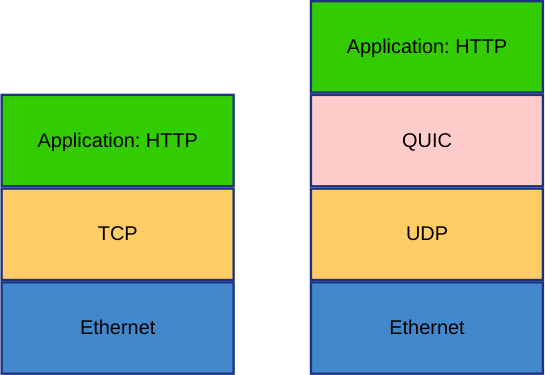
\includegraphics[height=0.20\textheight]{figures/network_layers.png}
    \caption{Modèle en couche - QUIC est construit sur UDP}
\end{figure}

Parmi les différences entre QUIC et TCP, on notera que QUIC chiffre toutes les communications, même les acquittements sont chiffrés de sorte que toute communication soit intégralement opaque pour un observateur extérieur. Un autre avantage majeur de QUIC est la possibilité de multiplexer différents flux sur une même connexion. En théorie cela permet de ne négocier la clef de chiffrement qu'une seule fois, réduisant ainsi la charge sur les serveurs HTTP/3. En effet, une simple recherche google génère aujourd'hui une cinquantaine de requêtes HTTP, chaque requête négociant une nouvelle clef de chiffrement. Intuitivement, pour des services comme YouTube, le nombre de requêtes est encore plus élevé, d'où l'intérêt de multiplexer les flux.
Pour finir sur les différences, QUIC apporte beaucoup plus de contrôle sur les paramètres de la connexion, permettant ainsi de le configurer pour des applications très différentes, du streaming haut débit sur YouTube à des connexions à très grande latence, comme une communication avec Mars.

Malgré tous ces avantages, QUIC a un défaut majeur, toutes les implémentations actuelles consomment énormément de puissance de calcul, bien plus que TCP.
Il y a plusieurs raisons à cela. D'une part, les implémentations de QUIC sont très jeunes et n'ont pas eu le temps d'être optimisées, contrairement aux implémentations de TCP qui ont reçu des décennies d'améliorations, l'implémentation de TCP dans Linux date de 1992\up{\cite{linux-first-tcp}}.
D'autre part, QUIC est fait pour être implémenté au-dessus d'UDP, du côté application, tandis que TCP est implémenté dans le kernel. Pour éviter que les trames IP soient fragmentées par les routeurs, les paquets que l'on génère ne doivent pas dépasser les 1400 octets. Travailler sur de si petits paquets rend la cryptographie plus intensive et nécessite de nombreux appels kernel, ce qui explique majoritairement les écarts de performances entre QUIC et TCP.

C'est pour contrebalancer ce défaut que beaucoup de recherches actuelles sur les implémentations de QUIC essayent de réduire l'utilisation du processeur par divers moyens, ce qui en pratique demande généralement d'ajouter des mécanismes dans le protocole QUIC pour traiter les données différemment.
QUIC VReverso et son implémentation frochet/quiceh est une de ces tentatives d'amélioration, l'idée étant ici de réduire le nombre de copies des données, ce qui consomme une part non négligeable du temps du processeur.

frochet/quiceh étant écrit en langage Rust, ne pouvait pas être intégré dans le client HTTP cURL qui est écrit en langage C. Il fallait donc écrire une FFI (Function to Function Interface), c'est à dire un morceau de code à l'interface entre les 2 langages qui convertit les données dans le format d'un langage vers le format de l'autre.
C'est le premier travail qui a été effectué.
\newpage

%------------ Travail effectué ----------------

\section{Travail effectué}
\subsection{Travail sur frochet/quiceh}

\subsubsection{Implémentation de la FFI}

Le code de frochet/quiceh est une bibliothèque, c'est-à-dire que ce code seul ne fait rien, il fournit seulement des fonctionnalités qui peuvent être utilisées dans d'autres programmes.
Un de ces programmes est cURL. cURL est un logiciel permettant d'effectuer des requêtes HTTP en ligne de commande. C'est un logiciel très important pour les développeurs sous Linux, car il est utilisé par des milliers d'autres logiciels.
cURL utilise cloudflare/quiche comme base pour effectuer des requêtes HTTP/3. Or Daniel Stenberg, le développeur principal de cURL se plaint régulièrement des performances d'HTTP/3\up{\cite{stenberg-complaining}}. Cela fait de cURL un choix parfait pour expérimenter le remplacement de cloudflare/quiche par frochet/quiceh et mesurer le gain de performances.

cURL est écrit en langage C tandis que frochet/quiceh est écrit en Rust, il a donc fallu écrire une FFI dans frochet/quiceh pour fournir à cURL une version C des fonctions de Quiceh.
On trouve près de 3500 fonctions dans le code de Quiceh; fort heureusement il n'est pas nécessaire d'écrire une interface C pour chaque fonction de Quiceh. Seules les fonctions utilisées par les programmes externes comme cURL doivent bénéficier d'une FFI, la plupart des fonctions sont des fonctions internes à Quiceh qui n'ont pas besoin d'interface C.
De plus, comme frochet/quiceh est dérivé du code de cloudflare/quiche, la plupart de la FFI était déjà écrite, il fallait écrire la FFI pour toutes les nouvelles fonctions de QUIC VReverso qui fonctionnent sans copie.

\begin{figure}[H]
    \centering
    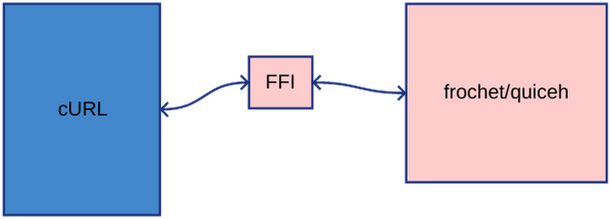
\includegraphics[height=0.15\textheight]{figures/curl_ffi_quiceh.png}
    \caption{La FFI est un morceau de code entre 2 projets écrits dans des langages différents}
\end{figure}

La FFI doit être écrite en langage Rust, n'ayant jamais fait de Rust auparavant, j'ai dû me former sur le langage et la syntaxe de ses FFI. Une fois ceci fait, j'ai pu rapidement écrire la dizaine de fonctions requises par cURL, en les testant non pas sur cURL mais sur un client HTTP très minimaliste en C que j'ai conçu pour l'occasion.

\subsubsection{Portage de frochet/quiceh dans cURL}

Une fois les fonctions de la FFI écrites dans frochet/quiceh, il fallait modifier le code de cURL pour les utiliser.
Malheureusement, cela ne pouvait se résumer à remplacer les fonctions de cloudflare/quiche par celles de frochet/quiceh. Le code de cURL n'était pas du tout conçu pour utiliser les interfaces zéro copie.
cURL copie tous les buffers qu'il reçoit et qu'il doit envoyer dans une queue interne. Si l'on utilise les fonctions de frochet/quiceh dans ce contexte, les données vont se retrouver corrompues car les buffers sont réutilisés.
On peut contourner le problème en copiant systématiquement les buffers dans de nouveaux avant de les ajouter à la queue, mais si l'on fait ça on déplace la copie depuis Quiche vers cURL au lieu de vraiment retirer cette copie.

\begin{figure}[H]
    \centering
    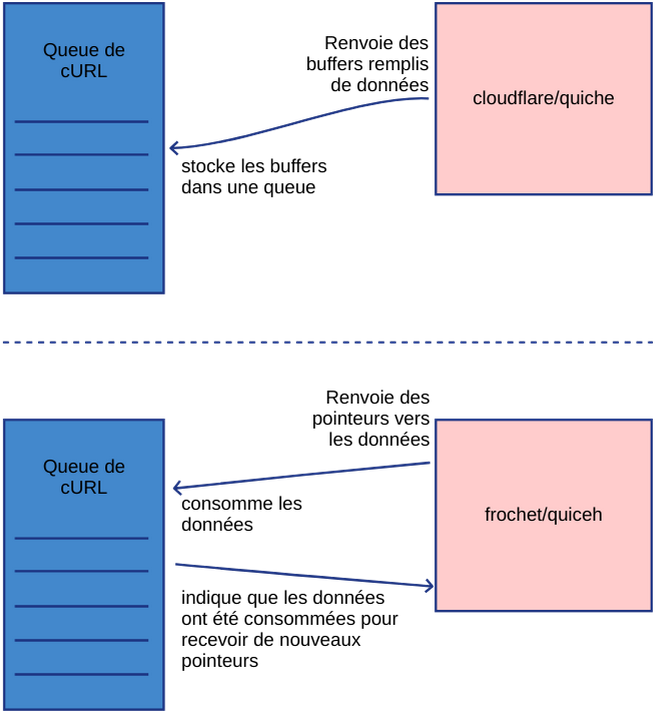
\includegraphics[height=0.37\textheight]{figures/curl_queue.png}
    \caption{\small{La différence de fonctionnement entre cloudflare/quiche et frochet/quiceh rend la queue de cURL inadaptée, car il faudrait copier les données pour les consommer.}}
\end{figure}

Pour mesurer un vrai gain de performance, la seule solution était de trouver un moyen de contourner la queue de cURL lorsqu'on utilise QUIC VReverso. A noter qu'il faut aussi garder l'ancienne queue et l'ancien fonctionnement pour le cas où le pair négocie QUIC V1 plutôt que QUIC VReverso.

\newpage

\subsection{Deuxième sous partie}

\subsubsection{A}

    \lipsum[1-2]

\subsubsection{B}

    \lipsum[1-2]
\newpage

%------------ Conclusion personnelle ----------------

\section{Conclusion personnelle}
\input{Chapters/conclusion_perso}
\newpage

%------------ Conclusion ----------------

\section{Conclusion} 
\input{Chapters/conclusion}
\newpage

%------------ Bibliographie ----------------

\printbibliography[heading=bibintoc, title={~~~~Bibliographie}]
\newpage

%------------ Annexe ----------------

\section{Annexe}
\input{Chapters/annexe}
\newpage

\end{document}
